% !TEX root=../dummy/dummy-06.tex

\chapter{双杂化泛函的静态极化率测评}
\label{sec.6.title}

\section{引言}

在上一章中,我们已经了解静态极化率的意义、其物理定义与计算策略、以及精确的理论计算极化率的具体实现方法。我们还注意到,静态极化率是现在机器学习方法在化学中应用的重要标准之一;许多机器学习方法都将静态极化率作为学习目标\cite{Ramakrishnan-Lilienfeld.SD.2014, Gilmer-Dahl.ICML.2017, Faber-Lilienfeld.JCTC.2017, Schuett-Mueller.NIPS.2017, Schuett-Mueller.JCP.2018, Wilkins-Ceriotti.PNAS.2019, Schuett-Gastegger.arXiv.2021, Zhang-Jiang.Elsevier.2023, Zou-Hu.NCS.2023}。作为二维张量,静态极化率是最基本的具有等变性的分子性质之一;因此对它的正确描述也可以验证机器学习网络的等变性、以及确认等变网络参数的有效性\cite{Cohen-Welling.arXiv.2016, Schuett-Gastegger.arXiv.2021, Brandstetter-Welling.arXiv.2022, Geiger-Smidt.arXiv.2022}。同时,作为参数化方法的学习目标,一些分子力学方法也对电子结构方法的极化率精确性有较高的需求\cite{Halgren-Damm.COSB.2001, Baker-Baker.WCMS.2015, Goloviznina-Padua.JCTC.2019, Schauperl-Gilson.CC.2020}。在大数据与 AI for Science 思潮盛行的时代,可信的、大通量高效的、精确的电子结构方法计算得到的静态极化率,将会、或已经成为亟待解决的重要需求。

尽管上一章中发展的 FPA 策略、以及其给出的 CCSD(T)/CBS 级别精确的极化率相当重要,但 CCSD(T) 计算消耗仍然十分巨大;若要将极化率计算应用到更大的体系,或者提升精确极化率计算的效率,则需要计算量更小的基组或电子结构方法。密度泛函近似在计算量与精度上,是普遍为计算化学与固体物理应用工作者所接受的方法;它有希望成为解决大量精确计算静态极化率问题的方法。

如第 \alertref{sec.1.title} 章所述,双杂化泛函已经在许多化学反应能量与分子性质的测评上,展现出良好的结果。如附录 \alertref{sec.3.title} 的所述,双杂化泛函的极化率计算尽管相比于杂化泛函更为耗时,但对于 2000 基组大小以内的中等体系是可以接受的,这也契合目前流行的诸多大数据集 20 重原子以内的分子大小\cite{Ruddigkeit-Reymond.JCIM.2012, Ramakrishnan-Lilienfeld.SD.2014, Bowman-Yu.JCP.2022, Zou-Hu.NCS.2023}。因此,双杂化泛函从计算效率上,应可以胜任静态极化率的大规模计算。对于偏重无机小分子与自旋极化分子的 HH132 数据集,Hait 与 Head-Gordon 的测评结果展示了双杂化泛函、特别是 xDH 型泛函静态极化率计算结果相当精确\cite{Hait-Head-Gordon.PCCP.2018}。

本章将拓展静态极化率测评结果,以更全面地展示密度泛函的精确性、以及如何高效但不失精度地计算静态极化率。在一定的、可容忍的误差范围内,使用合理大小的基组,可以有效地以较小的代价实现极化率的计算;\ref{sec.6.basis-converg} 节将对典型的双杂化泛函,B2PLYP 泛函与 xDH@B3LYP 类型泛函,在静态极化率问题上作基组误差分析,以探讨基组对计算精度的影响。目前基于高精度 CCSD(T)/CBS 精度的测评,仅涉及到少量双杂化泛函以及 HH132\cite{Hait-Head-Gordon.PCCP.2018} 为代表的小型无机分子;\ref{sec.6.benchmark} 节将基于第 \alertref{sec.5.title} 章的 CCSD(T)/CBS 精度的参考值,拓展数据集到 HR46\cite{Hickey-Rowley.JPCA.2014} 与 T144\cite{Wu-Thakkar.CPL.2015},测评包括更多双杂化泛函在内的诸密度泛函近似在静态极化率上的表现。对于分子性质的测评,最终应服务于密度泛函的发展;作为最初步的探索,\ref{sec.6.pol-xdh-optimize} 节将基于 xDH@B3LYP 参数化模型\cite{Zhang-Xu.JPCL.2021},仅针对极化率测评表现进行参数优化,探究 xDH@B3LYP 模式在极化率问题上的极限。

\section{实现细节}

本章工作继承第 \alertref{sec.5.title} 章工作;大多数实现细节上也参考 \alertref{sec.5.detail} 节。需要额外说明或有所不同的实现细节列出如下。

\subsection{数据集}

本章将测评 HR46\cite{Hickey-Rowley.JPCA.2014} 与 T144\cite{Wu-Thakkar.CPL.2015} 数据集。这两个数据集的 CCSD(T) 方法 FPA-aV[DT]Z、FPA-aV[TQ]Z 或 FPA-aV[Q5]Z 级别下计算得到的同性极化率 $\alpha$、异性极化率 $\gamma$ 的参考值已由表 \alertref{tab.5.s1}, \alertref{tab.5.s2}, \alertref{tab.5.s3}, \alertref{tab.5.s4} 给出。

本章工作也对 HH132 数据集\cite{Hait-Head-Gordon.PCCP.2018}的部分分子作测评与分析。由于诸多原因,HH132 中实际被测评的分子是 75 个自旋非极化分子、以及 26 个自旋极化分子,总共 101 个分子。详细说明见 \ref{sec.6.supp-HH132-remove} 节的讨论。本章后续将称该数据集为 HH101 数据集;对该数据集的误差讨论与分析中,将区分 26 个自旋极化 (SP) 与 75 个自旋非极化分子 (NSP)。该数据集的参考值是 CCSD(T) 方法 aCV[TQ]Z 或 aCV[Q5]Z 计算得到。

\subsection{电子结构计算}

本工作测评的极化率是解析梯度计算得到的结果。程序通过 \textsc{PySCF} (介于 2.1.0 到 2.4.0 版本)以及扩展程序脚本 \textsc{dh} (commit 80ca9e8) 实现。对于所有泛函,DFT 积分所使用的密度格点为第 4 级 (默认修剪、第一周期 (60, 434)、第二周期 (90, 590)、第三周期 (95, 590))。辅助基组均使用 ETB 自动生成基组。在极化率测评中,基组统一使用 aug-pc-3;在基组误差分析中,我们将使用 aCV$X$Z ($X = \mathrm{D, T, Q, 5}$) 与 aug-pc-$n$ ($n = 1, 2, 3, 4$) 基组;所使用到的 CBS 模型与 \alertref{sec.5.cbs} 节相同,且 CBS 外推仅针对相关贡献部分、而对自洽场部分不作外推。后续文段中,我们将简记基组 aug-pc-$n$ 为 apc$n$ ($n = 1, 2, 3, 4$)。

本工作测评并汇报 62 个密度泛函近似的极化率误差结果。被测评泛函分布如图 \ref{fig.6.pol-functionals-distribution} 所示。我们尽可能对目前流行的、且在 \textsc{dh} 程序中实现的双杂化泛函做极化率测评;涉及到 B95 的双杂化泛函由于部分体系存在收敛问题,本工作暂不纳入 \textsc{dh} 程序已经实现的 DSD-PBEB95-D3BJ 与 PWPB95-D3Zero 泛函;对于 ωB97X-2 泛函,我们仅测评其 TQZ 版本。本工作所涉及到的低阶泛函包括
\begin{itemize}[nosep]
    \item mBEEF, MVS, SCAN, MPW1K, PBE50, SCAN0, MPW91, N12 等泛函是 Hait 与 Head-Gordon 测评工作\cite{Hait-Head-Gordon.PCCP.2018}中表现较好的 GGA 或 mGGA 泛函;
    \item M11, M06-2X 是 T145 测评工作\cite{Wu-Thakkar.CPL.2015}中表现较好的泛函;
    \item PBE, BLYP, TPSS, N12, M06-L, B3LYP, PBE0, M06, TPSSh, MN15, CAM-B3LYP, ωB97M-V 等泛函是目前计算化学应用的常见泛函。
\end{itemize}
对于 ωB97M-V 泛函,本工作的计算不考虑其 VV10 贡献项。

我们同时对 HF、MP2、CCSD 的极化率表现作测评。对于 HH101 数据集,计算结果取自 Hait 与 Head-Gordon 的工作的 aCV[TQ]Z 或 aCV[Q5]Z 计算结果。对于 HR46 与 T144 数据集,计算结果取自第 \alertref{sec.5.title} 章工作;即 HF 与 MP2 使用 aCV[Q5]Z 计算结果,CCSD 使用 FPA-aV[DT]Z、FPA-aV[TQ]Z 或 FPA-aV[Q5]Z 计算结果。

\subsection{误差测评标准}

对于同性极化率 $\alpha$、异性极化率 $\gamma$ 的计算,我们将沿用式 \alertref{eq.5.relrmsd} 的 RelRMSD 误差量标。对于 HH101 数据集的测评,我们也对其极化率分量使用 RelRMSD 量标\footnote{HH132 原始文献\cite{Hait-Head-Gordon.PCCP.2018}中,Hait 等提出的误差量标是 RMSRE;若 RelRMSD 表达式 \alertref{eq.5.relrmsd} 的指标 $n$ 代表的不是分子、而是分子极化率的 $\alpha_{xx}, \alpha_{yy}, \alpha_{zz}$ 分量之一,那么 HH132 原始文献式 (3) 所表达的 RMSRE 与本工作的 RelRMSD 是等价的。但需要注意到,在 HH132 文献的 Supporting Information 中,Hait 等实际计算与汇报的误差是三个分量的平均值、而非方均根平均;即以 HH132 原始文献的记号,
$$
\text{RMSRE (reported)} = \frac{1}{3} \sum_{i=x,y,z} \sqrt{\frac{1}{N} \sum_{n=1}^N \varepsilon_{i,n}^2}
$$
这与 HH132 原文献的式 (3) 表述的方式有所不同;式 (3) 的具体表述是
\begin{equation}
    \label{eq.6.rmsre}
    \text{RMSRE (designed)} = \sqrt{\frac{1}{3N} \sum_{i=x,y,z} \sum_{n=1}^N \varepsilon_{i,n}^2}
\end{equation}
尽管一般来说两者数值上非常接近、且几乎不会影响泛函测评表现。在本工作中,我们使用 HH132 原文献式 (3) 的表述、或者等价地使用 RelRMSD 对数据集的极化率分量 $\alpha_{xx}, \alpha_{yy}, \alpha_{zz}$ 作测评。
}。

由于我们将测评多种数据集以及多种类型的极化率;为简化分析,这里定义加权相对误差 WTRE (weighted relative error) 以对泛函的总体极化率误差进行合适的排序。对于数据集以及其对应的测评性质 $d$,泛函 $f$ 的相对方均根误差 RelRMSD 的测评结果 $\epsilon_{f,d}$,泛函的加权相对误差是
\begin{equation}
    \label{eq.6.wtre}
    \mathrm{WTRE}_f = \sum_d w_d \epsilon_{f,d}
\end{equation}
具体的测评性质 $d$、以及权重 $w_d$ 定义如表 \ref{tab.6.benchmark-weight} 所示。WTRE 是无量纲量,也并非百分比误差。权重 $w_d$ 定义为反比于本工作所测评泛函平均 RelRMSD 误差的量:
\begin{equation}
    w_d = \frac{1}{\mathrm{count} \{ d \}} \frac{1}{\mathrm{count} \{ f \}} \frac{1}{\displaystyle \sum_{f} \epsilon_{f,d}}
\end{equation}
其中,$\mathrm{count} \{ d \} = 8$ 是指 8 个被测评的性质 (参考表 \ref{tab.6.benchmark-weight}),$\mathrm{count} \{ f \}$ 是指被测评的 64 个泛函 (参考图 \ref{fig.6.pol-functionals-distribution})。在此定义下,本工作所测评的泛函 WTRE 误差的平均值是 1,即
\begin{equation*}
    \frac{1}{\mathrm{count} \{ f \}} \sum_f \mathrm{WTRE}_f = 1
\end{equation*}
若泛函 $f$ 所对应的加权误差 $\mathrm{WTRE}_f$ 越小,则泛函 $f$ 的总体极化率表现越好;若 $\mathrm{WTRE}_f$ 接近 1,则表明泛函 $f$ 的测评表现处于平均水平。

\begin{figure}[t]
    \centering
    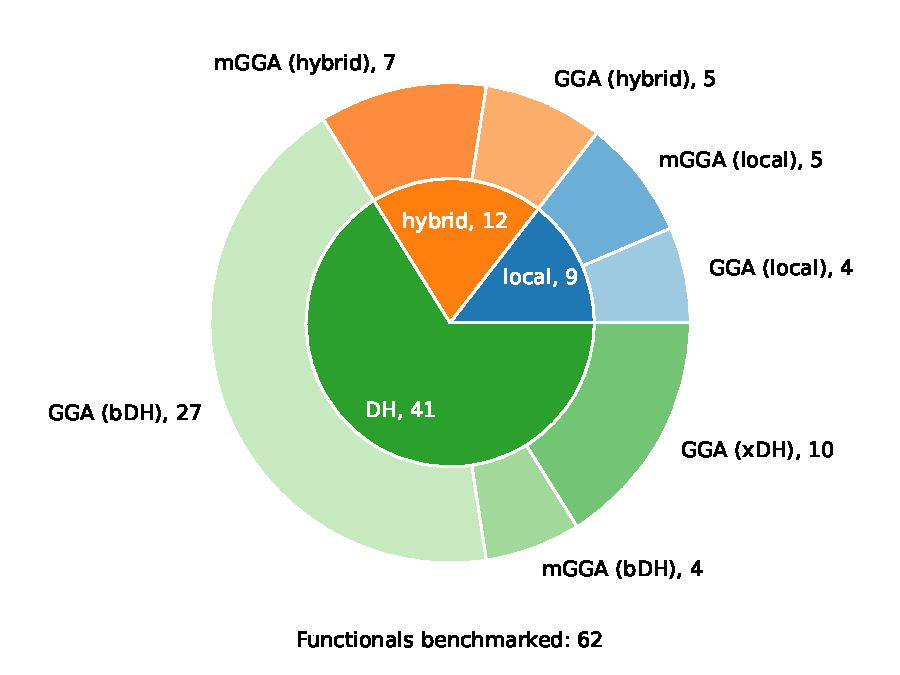
\includegraphics[width=0.6\textwidth]{assets/pol-functionals-distribution.pdf}
    \caption[静态极化率测评泛函的大致分类与数量示意图]{本工作测评泛函的大致分类与数量示意图。}
    \label{fig.6.pol-functionals-distribution}
\end{figure}

\begin{table}[!ht]
\centering
\caption[静态极化率测评权重表]{静态极化率测评权重表。}
\label{tab.6.benchmark-weight}
\widetabular{
    \begin{tabular}{lld{3.8}}
    \toprule
    性质        & 数据集 ($d$) & \multicolumn{1}{c}{权重 ($w_d$)} \\ \midrule
    同性极化率  & HR46        & 0.0618371 \\
                & T144        & 0.0548781 \\
                & HH101 (NSP) & 0.0382151 \\
                & HH101 (SP)  & 0.0326924 \\ \midrule
    异性极化率\tnote{a} & HR46        & 0.0245850 \\
                & T144        & 0.0250915 \\ \midrule
    极化率分量  & HH101 (NSP) & 0.0370998 \\
                & HH101 (SP)  & 0.0298901 \\ \bottomrule
    \end{tabular}
}{
    \item[a] 部分分子异向极化率 $\gamma$ 小于 0.5 \AA${}^3$,不适合作相对误差分析;因此对于异向极化率,HR46 数据集总共测评 39 个分子 (除去 \ce{H2O}, \ce{CH4}, \ce{CH3F}, \ce{PH2}, \ce{H2S}, \ce{SiH4}, \ce{NH3} 共七个分子),T144 数据集总共测评 141 个分子 (除去 0351 \ce{C2H5F}, 0353 \ce{CH3F}, 0998 \ce{CF3CHF2} 共三个分子)。
}
\end{table}

\subsection{泛函参数优化}

本工作将会简要地考察泛函的参数调整问题。我们选用 \textsc{SciPy}\cite{Virtanen-Vazquez-Baeza.NM.2020} 进行泛函参数的优化。优化算法选用 L-BFGS-B 算法\cite{Byrd-Zhu.SJSC.1995},收敛判标是参数梯度模长 (\verb|gtol|) 小于 $10^{-5}$。我们采用简单的全局优化方法,即在优化后的泛函参数上施加不超过 0.5 的随机参数系数再次优化,反复 20 次,并汇报取得最低 $\mathrm{WTRE}_f$ 时的泛函参数。

\section{典型双杂化泛函静态极化率基组误差分析}
\label{sec.6.basis-converg}

这一节中,我们将以典型的双杂化泛函 B2PLYP 作为例子,分析其静态极化率的基组误差。

对于 B2PLYP 而言,其同性极化率 $\alpha_\textsf{DH}$ 可以分解为自洽场部分 $\alpha_\textsf{SCF}$ 与二阶微扰部分 $\symup{\Delta} \alpha_\textsf{PT}$ 之和
\begin{equation*}
    \alpha_\textsf{DH} = \alpha_\textsf{SCF} + \symup{\Delta} \alpha_\textsf{PT2} \quad \text{(B2PLYP-like doubly hybrid)}
\end{equation*}
我们将对这两部分分量,分别作基组收敛分析。作为基准,我们选取 aCV[Q5]Z 的 CBS 外推模型作为参考值;这也与第 \alertref{sec.5.title} 章的最佳 CBS 外推标准相同:
\begin{equation*}
    \alpha_\textsf{DH} (\text{aCV[Q5]Z}) = \alpha_\textsf{SCF} (\text{aCV5Z}) + \symup{\Delta} \alpha_\textsf{PT2} (\text{aCV[Q5]Z})
\end{equation*}
对于其他 CBS 外推模式下的双杂化泛函极化率,其自洽场部分将使用较大的基组结果、而二阶微扰部分将采用 CBS 外推:
\begin{align*}
    \alpha_\textsf{DH} (\text{aCV}[XY]\text{Z}) &= \alpha_\textsf{SCF} (\text{aCV}Y\text{Z}) + \symup{\Delta} \alpha_\textsf{PT2} (\text{aCV}[XY]\text{Z}) \; &&([XY] = \mathrm{[DT], [TQ]}) \\
    \alpha_\textsf{DH} (\text{apc}[nm]) &= \alpha_\textsf{SCF} (\text{apc}m) + \symup{\Delta} \alpha_\textsf{PT2} (\text{apc}[nm]) \; &&([nm] = [12], [23], [34])
\end{align*}
对于异性极化率 $\gamma_\textsf{DH}$ 也可以作类似的拆解。

\subsection{HR46 与 T144 数据集分析}

HR46 与 T144 大多数分子为有机分子、且分子大小较大,两个数据集较为相近。表 \ref{tab.6.b2p-conv-hr46-t144-iso} 与表 \ref{tab.6.b2p-conv-hr46-t144-aniso} 分别展示了 HR46 与 T144 数据集下 B2PLYP 在同性极化率 $\alpha$ 与异性极化率 $\gamma$ 下的基组收敛性表现。

\begin{table}[!ht]
\centering
\caption[B2PLYP 在 HR46 与 T144 下同性极化率 $\alpha$ 的基组 RelRMSD]{B2PLYP 在数据集 HR46 与 T144 下同性极化率 $\alpha$ 的基组相对方均根误差 (RelRMSD / \%)${}^a$。}
\label{tab.6.b2p-conv-hr46-t144-iso}
\widetabular{
    \begin{tabular}{cld{1.3}d{1.3}d{1.3}d{1.3}d{1.3}d{1.3}}
    \toprule
    & & \multicolumn{3}{c}{HR46} & \multicolumn{3}{c}{T144} \\
    \cmidrule(lr){3-5} \cmidrule(lr){6-8}
    基组基数 & 基组 & \multicolumn{1}{c}{$\tilde \alpha_\textsf{SCF}$\tnote{b}} & \multicolumn{1}{c}{$\symup{\Delta} \tilde \alpha_\textsf{PT2}$\tnote{c}} & \multicolumn{1}{c}{$\tilde \alpha_\textsf{DH}$\tnote{d}} & \multicolumn{1}{c}{$\tilde \alpha_\textsf{SCF}$} & \multicolumn{1}{c}{$\symup{\Delta} \tilde \alpha_\textsf{PT2}$} & \multicolumn{1}{c}{$\tilde \alpha_\textsf{DH}$} \\
    \midrule
    2-$\zeta$ & aCVDZ    & 2.428 & 0.250 & 2.528 & 1.560 & 0.185 & 1.448 \\
              & apc1     & 1.001 & 0.188 & 0.905 & 0.855 & 0.225 & 0.686 \\ \midrule
    3-$\zeta$ & aCVTZ    & 0.542 & 0.120 & 0.571 & 0.241 & 0.134 & 0.152 \\
              & apc2     & 0.262 & 0.144 & 0.187 & 0.222 & 0.166 & 0.099 \\
              & aCV[DT]Z &       & 0.111 & 0.532 &       & 0.124 & 0.146 \\
              & apc[12]  &       & 0.153 & 0.224 &       & 0.150 & 0.114 \\ \midrule
    4-$\zeta$ & aCVQZ    & 0.086 & 0.069 & 0.121 & 0.018 & 0.082 & 0.073 \\
              & apc3     & 0.067 & 0.061 & 0.120 & 0.029 & 0.078 & 0.104 \\
              & aCV[TQ]Z &       & 0.057 & 0.096 &       & 0.049 & 0.041 \\
              & apc[23]  &       & 0.029 & 0.073 &       & 0.019 & 0.044 \\ \midrule
    5-$\zeta$ & aCV5Z    & \multicolumn{1}{c}{0\tnote{e}} & 0.036 & 0.036 & \multicolumn{1}{c}{0\tnote{e}} & 0.042 & 0.042 \\
              & apc4     & 0.099 & 0.046 & 0.140 & 0.050 & 0.054 & 0.102 \\
              & aCV[Q5]Z &       & \multicolumn{1}{c}{0\tnote{e}} & \multicolumn{1}{c}{0\tnote{e}} &       & \multicolumn{1}{c}{0\tnote{e}} & \multicolumn{1}{c}{0\tnote{e}} \\
              & apc[34]  &       & 0.034 & 0.127 &       & 0.032 & 0.080 \\
    \bottomrule
    \end{tabular}
}{
    \item[a] 该表格的部分数值因为选取为参考值,因此 $\tilde \alpha_\textsf{SCF}$ 在 aCV5Z、$\symup{\Delta} \tilde \alpha_\textsf{PT2}$ 与 $\tilde \alpha_\textsf{DH}$ 在 aCV[Q5]Z 下的误差值严格为零。
    \item[b] 自洽场部分同性极化率相对方均根误差为 $\text{RelRMSD} (\tilde \alpha_{\textsf{SCF}/\text{basis}}, \tilde \alpha_{\textsf{SCF}/\text{ref}}, \tilde \alpha_{\textsf{DH}/\text{ref}})$。其中,$\tilde \alpha_{\textsf{SCF}/\text{ref}}$ 指代的是大基组的 $\tilde \alpha_{\textsf{SCF}/\text{aCV5Z}}$,$\tilde \alpha_{\textsf{DH}/\text{ref}}$ 指代的是作为大基组参考值的 $\tilde \alpha_{\textsf{DH}/\text{aCV[Q5]Z}}$。
    \item[c] 二阶微扰部分同性极化率相对方均根误差为 $\text{RelRMSD} (\symup{\Delta} \tilde \alpha_{\textsf{PT2}/\text{basis}}, \symup{\Delta} \tilde \alpha_{\textsf{PT2}/\text{ref}}, \tilde \alpha_{\textsf{DH}/\text{ref}})$。其中,$\symup{\Delta} \tilde \alpha_{\textsf{PT2}/\text{ref}}$ 指代的是大基组的 $\symup{\Delta} \tilde \alpha_{\textsf{PT2}/\text{aCV[Q5]Z}}$。
    \item[d] 双杂化总同性极化率相对方均根误差为 $\text{RelRMSD} (\tilde \alpha_{\textsf{DH}/\text{basis}}, \tilde \alpha_{\textsf{DH}/\text{ref}})$。
    \item[e] 这些数值依据参考值的选取方式,从定义上是零。
}
\end{table}

\begin{table}[!ht]
\centering
\caption[B2PLYP 在 HR46 与 T144 下异性极化率 $\gamma$ 的基组 RelRMSD]{B2PLYP 在数据集 HR46 与 T144 下异性极化率 $\gamma$ 的基组相对方均根误差 (RelRMSD / \%)${}^a$。}
\label{tab.6.b2p-conv-hr46-t144-aniso}
\widetabular{
    \begin{tabular}{cld{1.3}d{1.3}d{1.3}d{1.3}d{1.3}d{1.3}}
    \toprule
    & & \multicolumn{3}{c}{HR46} & \multicolumn{3}{c}{T144} \\
    \cmidrule(lr){3-5} \cmidrule(lr){6-8}
    基组基数 & 基组 & \multicolumn{1}{c}{$\tilde \gamma_\textsf{SCF}$} & \multicolumn{1}{c}{$\symup{\Delta} \tilde \gamma_\textsf{PT2}$} & \multicolumn{1}{c}{$\tilde \gamma_\textsf{DH}$} & \multicolumn{1}{c}{$\tilde \gamma_\textsf{SCF}$} & \multicolumn{1}{c}{$\symup{\Delta} \tilde \gamma_\textsf{PT2}$} & \multicolumn{1}{c}{$\tilde \gamma_\textsf{DH}$} \\
    \midrule
    2-$\zeta$ & aCVDZ    & 3.389 & 0.505 & 3.596 & 1.742 & 0.264 & 1.860 \\
              & apc1     & 2.271 & 0.892 & 2.885 & 1.321 & 0.446 & 1.530 \\ \midrule
    3-$\zeta$ & aCVTZ    & 0.777 & 0.122 & 0.845 & 0.313 & 0.090 & 0.374 \\
              & apc2     & 0.342 & 0.311 & 0.503 & 0.159 & 0.145 & 0.201 \\
              & aCV[DT]Z &       & 0.230 & 0.845 &       & 0.137 & 0.383 \\
              & apc[12]  &       & 0.130 & 0.351 &       & 0.103 & 0.170 \\ \midrule
    4-$\zeta$ & aCVQZ    & 0.140 & 0.073 & 0.196 & 0.053 & 0.059 & 0.090 \\
              & apc3     & 0.102 & 0.124 & 0.174 & 0.061 & 0.058 & 0.085 \\
              & aCV[TQ]Z &       & 0.058 & 0.183 &       & 0.043 & 0.079 \\
              & apc[23]  &       & 0.099 & 0.115 &       & 0.050 & 0.055 \\ \midrule
    5-$\zeta$ & aCV5Z    & \multicolumn{1}{c}{0} & 0.038 & 0.038 & \multicolumn{1}{c}{0} & 0.030 & 0.030 \\
              & apc4     & 0.108 & 0.053 & 0.130 & 0.061 & 0.038 & 0.073 \\
              & aCV[Q5]Z &       & \multicolumn{1}{c}{0} & \multicolumn{1}{c}{0} &       & \multicolumn{1}{c}{0} & \multicolumn{1}{c}{0} \\
              & apc[34]  &       & 0.041 & 0.122 &       & 0.037 & 0.071 \\
    \bottomrule
    \end{tabular}
}{
    \item[a] 该表格的图例参考表 \ref{tab.6.b2p-conv-hr46-t144-iso}。
}
\end{table}

可以看到,若不考虑计算量相当大的 5-$\zeta$ 基组或 CBS 方法,对于双杂化泛函总极化率 $\alpha_\textsf{DH}$ 或 $\gamma_\textsf{DH}$,Jensen 基组 apc$n$ ($n = 1, 2, 3$) 通常比 Dunning 基组 aCV$X$Z ($X = \mathrm{D, T, Q}$) 在相同的基组基数 $\zeta$ 下,有更低的误差 (例外是 T144 数据集 4-$\zeta$ 下同性极化率 $\alpha_\textsf{DH}$ 的相对方均根误差)。而同时注意到,对于相同的基组基数 $\zeta$,Jensen 基组 apc$n$ 的大小通常小于 Dunning 基组 aCV$X$Z;因此对于 2,3,4-$\zeta$ 的情形,Jensen 基组 apc$n$ 在极化率计算问题上,不论是性能需求还是误差都要好于 Dunning 基组 aCV$X$Z。

在 \alertref{sec.5.bench-wft-polar} 小节对小分子体系 MP2 极化率的基组误差分析中,HF 方法的极化率 $\alpha_\textsf{HF}$ 与 $\gamma_\textsf{HF}$ 的误差,随着基组基数 $\zeta$ 的增大而快速减小。而相对地,MP2 的相关贡献 $\symup{\Delta} \alpha_\textsf{(2)}$ 与 $\symup{\Delta} \gamma_\textsf{(2)}$ 的收敛趋势较慢;对于同性极化率 $\symup{\Delta} \alpha_\textsf{(2)}$ 的误差在 4,5-$\zeta$ 下远远大于 $\alpha_\textsf{HF}$。而对于 HR46 与 T144 数据集的 B2PLYP 计算下,二阶微扰贡献 $\symup{\Delta} \alpha_\textsf{PT2}$ 与 $\symup{\Delta} \gamma_\textsf{PT2}$ 的误差相比于自洽场部分 $\alpha_\textsf{SCF}$ 与 $\gamma_\textsf{SCF}$ 一般来说相当或更小。注意到 B2PLYP 泛函的二阶微扰贡献系数 $c_\textmt{c} = 0.27$,因此尽管二阶微扰本身的收敛趋势较慢、但在系数的缩放下并没有体现出很大的误差。

对于 Jensen 基组 apc$n$,其计算同性极化率 $\alpha_\textsf{DH}$ 时,apc2 的误差已经小于 0.2\%;甚至在 T144 数据集下 $\alpha_\textsf{DH}$ 的相对方均根误差为 0.099\%,比之计算代价更大的 apc3 基组的误差更小。但同时考虑到构成 $\alpha_\textsf{DH}$ 的两个分项 $\alpha_\textsf{SCF}$ 与 $\symup{\Delta} \alpha_\textsf{PT2}$,apc2 在这两个分项的误差远远大于 apc3。因此,apc2 同性极化率 $\alpha_\textsf{DH}$ 相当小的误差,应当归因于 $\alpha_\textsf{SCF}$ 与 $\symup{\Delta} \alpha_\textsf{PT2}$ 误差的相互抵消,而不应认为其同性极化率 $\alpha_\textsf{DH}$ 已经接近基组极限;考虑到其他双杂化泛函的构造与 B2PLYP 有所不同,apc2 的 $\alpha_\textsf{DH}$ 计算结果未必能保证对 B2PLYP 以外的其他双杂化泛函有稳定的低误差。

CBS 外推模型在 4-$\zeta$ 的基组基数下有较好的效果:相对于单一基组 aCVQZ 或 apc3 计算,CBS 外推的 aCV[TQ]Z 或 apc[23] 的误差有所降低。对于 3-$\zeta$ 下,CBS 外推与否对同性极化率 $\symup{\Delta} \alpha_\textsf{PT2}$ 影响较小;而对异性极化率 $\symup{\Delta} \gamma_\textsf{PT2}$,Dunning 基组 aCV[DT]Z 的误差比 aCVTZ 误差大、但 Jensen 基组 apc[12] 的误差比 apc2 小。值得注意的是,apc[12] 的同性极化率误差比 $\symup{\Delta} \alpha_\textsf{PT2}$ 小、但 $\alpha_\textsf{DH}$ 的误差反而更大;即每个极化率贡献项分别更小的误差,反而在总和的结果上给出更大的误差;这也印证了 apc2 较低的 $\alpha_\textsf{DH}$ 误差不能表明 apc2 本身的误差很小。

尽管 CBS 外推模型在 4-$\zeta$ 基组基数有良好表现,但注意到 4-$\zeta$ 基组 aCVQZ、apc3 本身的计算误差也仅有不到 0.2\%,CBS 外推的优势比较有限。因此,我们认为对于 HR46 与 T144 数据集,使用 4-$\zeta$ 基组 aCVQZ、apc3 进行双杂化泛函的计算,误差较低且远低于实验误差的 0.5\%,是适合用于测评的基组。而对于 3-$\zeta$,若分别考察 $\alpha_\textsf{SCF}$ 与 $\symup{\Delta} \alpha_\textsf{PT2}$ 分别的误差并作加和,则对于 HR46 数据集的 aCVTZ 或 aCV[DT]Z 误差在 0.65\% 左右,HR46 数据集的 apc2 或 apc[12]、以及 T144 数据集的 3-$\zeta$ 基组或 CBS 外推模型的误差在 0.40\% 左右。apc2 或 apc[12] 的误差尽管小于实验误差的 0.5\%,但幅度不是很大。我们认为,apc2 或 apc[12] 也是可以接受的;但在计算量可接受的情形下,应尽可能使用 4-$\zeta$ 基组或 CBS 外推模型。

最后,我们指出,表 \ref{tab.6.b2p-conv-hr46-t144-iso} 与表 \ref{tab.6.b2p-conv-hr46-t144-aniso} 的数据将表明 5-$\zeta$ 情形下 Jensen 基组 apc4 与 apc[34] 的误差普遍比 Dunning 基组 aCV5Z 更大;并且尽管 apc4 与 apc[34] 计算代价更大,其误差并未比 apc3 与 apc[23] 更进步、甚至误差更大。对此,我们认为,5-$\zeta$ 情形下 Jensen 基组与 Dunning 基组之间的误差反映的是 5-$\zeta$ 级别基组的基组不完备程度;这个不完备程度一般小于 0.2\%,且远小于 0.5\% 的实验误差,这是完全可以接受的误差范围。除此之外,这里作 B2PLYP 基组误差分析的目的,是确认一种在可接受误差的前提下计算效率更高的基组、以及确定基组误差对双杂化泛函测评的影响;当基组达到 4-$\zeta$ 或更大时,其极化率相对误差已经远小于 0.5\%,不会对泛函测评的结果产生明显影响。关于 5-$\zeta$ 级别基组或 CBS 外推方法精度的更多分析,我们在附录 \ref{sec.6.supp-bsie} 小节中展开。

\subsection{HH101 数据集分析}

HH101 数据集包含的分子或原子较小、且有机分子很少;其数据集构成与 HR46 与 T144 有较大差异。表 \ref{tab.6.b2p-conv-hh101-iso} 展示了 HH101 数据集下 B2PLYP 在同性极化率 $\alpha$ 下的基组收敛性表现。

\begin{table}[!ht]
\centering
\caption[B2PLYP 在 HH101 下同性极化率 $\alpha$ 的基组 RelRMSD]{B2PLYP 在数据集 HH101 下同性极化率 $\alpha$ 的基组相对方均根误差 (RelRMSD / \%)${}^a$。}
\label{tab.6.b2p-conv-hh101-iso}
\widetabular{
    \begin{tabular}{cld{1.3}d{1.3}d{1.3}d{1.3}d{1.3}d{1.3}}
    \toprule
    & & \multicolumn{3}{c}{HH101 (NSP)\tnote{b}} & \multicolumn{3}{c}{HH101 (SP)} \\
    \cmidrule(lr){3-5} \cmidrule(lr){6-8}
    基组基数 & 基组 & \multicolumn{1}{c}{$\tilde \alpha_\textsf{SCF}$} & \multicolumn{1}{c}{$\symup{\Delta} \tilde \alpha_\textsf{PT2}$} & \multicolumn{1}{c}{$\tilde \alpha_\textsf{DH}$} & \multicolumn{1}{c}{$\tilde \alpha_\textsf{SCF}$} & \multicolumn{1}{c}{$\symup{\Delta} \tilde \alpha_\textsf{PT2}$} & \multicolumn{1}{c}{$\tilde \alpha_\textsf{DH}$} \\
    \midrule
    2-$\zeta$ & aCVDZ    & 4.565 & 0.569 & 4.939 & 3.721 & 0.746 & 4.030 \\
              & apc1     & 1.783 & 0.882 & 1.991 & 1.642 & 0.944 & 1.800 \\ \midrule
    3-$\zeta$ & aCVTZ    & 1.358 & 0.294 & 1.568 & 0.866 & 0.325 & 1.006 \\
              & apc2     & 0.508 & 0.334 & 0.450 & 0.622 & 0.618 & 0.693 \\
              & aCV[DT]Z &       & 0.218 & 1.469 &       & 0.213 & 0.916 \\
              & apc[12]  &       & 0.550 & 0.578 &       & 0.500 & 0.605 \\ \midrule
    4-$\zeta$ & aCVQZ    & 0.302 & 0.150 & 0.432 & 0.146 & 0.205 & 0.282 \\
              & apc3     & 0.196 & 0.109 & 0.248 & 0.167 & 0.143 & 0.190 \\
              & aCV[TQ]Z &       & 0.070 & 0.344 &       & 0.161 & 0.219 \\
              & apc[23]  &       & 0.257 & 0.329 &       & 0.224 & 0.344 \\ \midrule
    5-$\zeta$ & aCV5Z    & \multicolumn{1}{c}{0} & 0.077 & 0.077 & \multicolumn{1}{c}{0} & 0.105 & 0.105 \\
              & apc4     & 0.216 & 0.075 & 0.256 & 0.136 & 0.112 & 0.190 \\
              & aCV[Q5]Z &       & \multicolumn{1}{c}{0} & \multicolumn{1}{c}{0} &       & \multicolumn{1}{c}{0} & \multicolumn{1}{c}{0} \\
              & apc[34]  &       & 0.155 & 0.283 &       & 0.094 & 0.177 \\
    \bottomrule
    \end{tabular}
}{
    \item[a] 该表格的图例参考表 \ref{tab.6.b2p-conv-hr46-t144-iso}。
    \item[b] 由于氢原子在 \textsc{dh} 程序中无法给出解析极化率,因此分析自旋非极化分子总体误差时排除氢原子,即总共分析 74 个自旋非极化体系。
}
\end{table}

可以看到,在相同的基组大小下,HH101 数据集的基组误差相比于 HR46 或 T144 数据集有更大的误差。以 4-$\zeta$ 级别基组来看,HR46 与 T144 数据集同性极化率对于 aCVQZ 与 apc3、以及对应的 CBS 外推模型下,$\alpha_\textsf{SCF}$ 与 $\symup{\Delta} \alpha_\textsf{PT2}$ 的相对方均根误差之和普遍在 0.15\% 以内;但在 HH101 数据集中,aCVQZ 在自旋非极化的 74 个分子中,其 $\alpha_\textsf{SCF}$ 与 $\symup{\Delta} \alpha_\textsf{PT2}$ 的相对方均根误差之和可以达到 0.45\%;apc3 的误差也达到 0.31\%;这表明 apc3 基组的误差仍然可以接受,但已经比较接近实验误差的 0.5\%。

需要指出,即使到 5-$\zeta$ 级别,apc4 基组 $\alpha_\textsf{SCF}$ 与 $\symup{\Delta} \alpha_\textsf{PT2}$ 的相对方均根误差之和也达到了 0.29\%,意味着我们所测评的最高等级基组之间也存在不能完全忽视的相对误差;这应归因于 5-$\zeta$ 级别基组的 BSIE。

若不考虑 CBS 外推模型,与 HR46、T144 数据集在 4-$\zeta$ 下 $\alpha_\textsf{SCF}$ 比起 $\symup{\Delta} \alpha_\textsf{PT2}$ 相对方均根误差较为接近或者更小的情况不同,HH101 数据集即使基组达到了 4-$\zeta$ 的较大级别,$\alpha_\textsf{SCF}$ 仍然具有一定的相对误差、且数值上与 $\symup{\Delta} \alpha_\textsf{PT2}$ 的相对误差接近或更大。

作为表 \ref{tab.6.b2p-conv-hh101-iso} 的补充,在本章附录中,表 \ref{tab.6.b2p-conv-hh101-rmsre} 的测评数据引入了非同性的效应,展示了极化率分量 $\alpha_{xx}$, $\alpha_{yy}$, $\alpha_{zz}$ 下的基组收敛性表现。从数据数值来看,HH101 数据集 B2PLYP 双杂化泛函下极化率分量的基组收敛性与同性极化率的基组收敛性表现相近;因此,上述分析对于非同性的电子极化效应仍然适用。

\subsection{基组误差分析小结}

这一节中,我们对 B2PLYP 双泛函的基组收敛性作了分析。我们认为,对于所有本工作所涉及的数据集 (HH101, HR46, T144)、在同性极化率 $\alpha$ 与异性极化率 $\gamma$ 上,4-$\zeta$ 基组可以同时在自洽场部分 $\alpha_\textsf{SCF}$, $\gamma_\textsf{SCF}$ 与二阶微扰部分 $\symup{\Delta} \alpha_\textsf{PT2}$, $\symup{\Delta} \gamma_\textsf{PT2}$ 稳定地达到不大于 0.5\% 的误差。在 4-$\zeta$ 级别的基组或 CBS 外推模型中,apc3 基组不仅误差相对较低、其基组大小也相对较小;使用 apc3 精确地计算静态极化率是性价比相对较高的计算方式。

B2PLYP 是典型的双杂化泛函;其他各式各色双杂化泛函的严格交换能杂化系数 $c_\textmt{x}$ 与二阶微扰相关能杂化系数 $c_\textmt{c}$ 与 B2PLYP 相对接近,因此可以预期其他双杂化泛函将有类似的基组误差表现。下一节的泛函静态极化率测评中,我们将统一使用 apc3 基组。

上述分析中,我们没有非常细致地分析不同 5-$\zeta$ 基组或 CBS 外推模型的误差。我们认为这很有可能是作为参考值的 aCV[Q5]Z 仍然存在一定的 BSIE;但由于更大基组计算上存在困难、一些基组系列欠缺更大的 Gaussian 函数型基组 (如目前没有标准的 aug-cc-pCV6Z 基组)、以及我们尚未掌握更精确的双杂化泛函的非 Gaussian 函数型基组解析极化率计算方法\cite{Brakestad-Frediani.JCTC.2020},因此目前无法在更高的基组精度上做严格的 BSIE 分析。我们猜测,在考虑 5-$\zeta$ 级别基组或 CBS 外推方法 BSIE 的前提下,上述基组误差分析的结论仍然成立、apc3 基组的误差将不会严重影响双杂化泛函的测评。更多关于 BSIE 误差的推测与推论,参考附录 \ref{sec.6.supp-bsie} 的讨论。

\section{密度泛函的静态极化率测评}
\label{sec.6.benchmark}

这一节对诸多密度泛函在静态极化率上的测评表现作讨论。详细的测评数据在附录的表 \ref{tab.6.full-benchmark} 中呈现;这里将对该表格数据作整理与分析。

\subsection{总体误差测评与讨论}

\begin{figure}[!t]
    \centering
    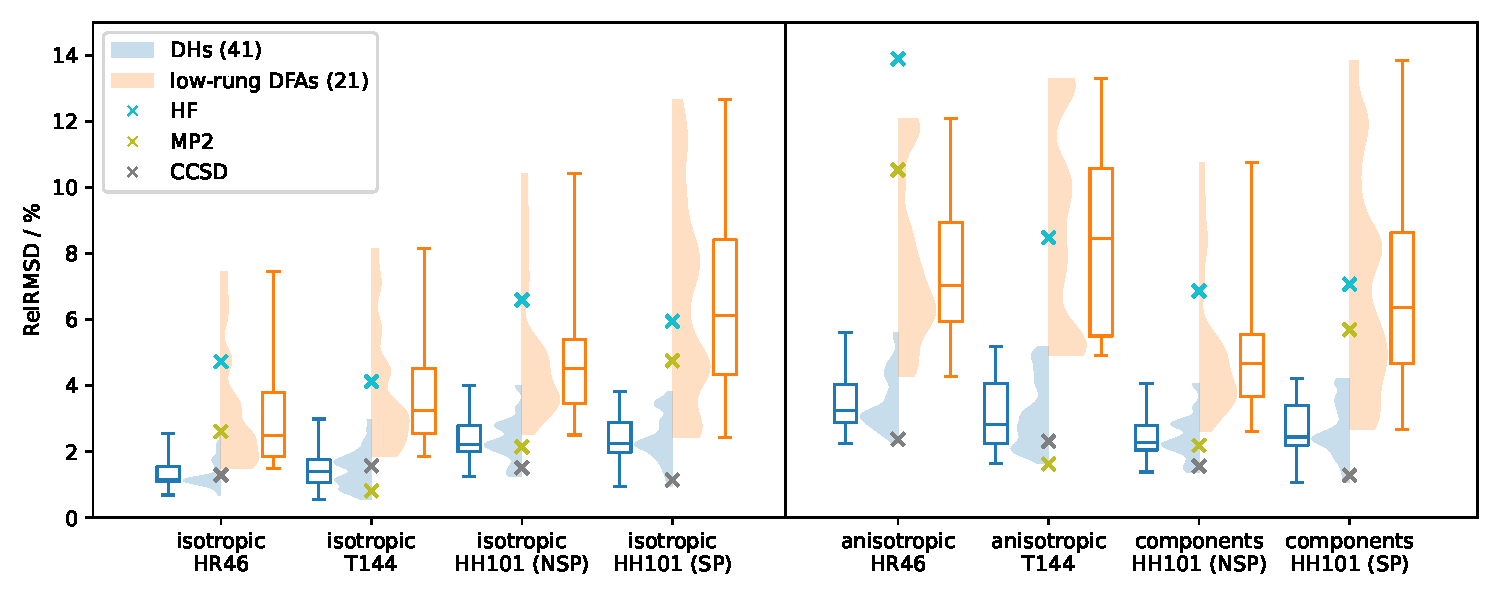
\includegraphics[width=0.8\textwidth]{assets/benchmark-compare-dh-low.pdf}
    \caption[诸泛函极化率 RelRMSD 测评表现图]{诸双杂化泛函 (DH) 与诸低阶泛函 (low-rung DFA) 泛函极化率数据集相对方均根误差 (RelRMSD) 测评表现图。小提琴图的数据密度建模方式是 Gaussian 核,参数 \texttt{bw\_method} 设为 0.2。箱型图展示了密度泛函测评误差的 1/4 位次、中位次、3/4 位次误差。图例中括号数字表示其对应分类被测评的泛函数量。}
    \label{fig.6.benchmark-compare-dh-low}
\end{figure}

首先对所有泛函总体表现作简要的测评。图 \ref{fig.6.benchmark-compare-dh-low} 展示了双杂化泛函与低阶泛函的总体误差表现、以及这两者之间的对比情况:
\begin{itemize}[nosep]
    \item 对于所有泛函,HR46 与 T144 数据集的异性极化率 $\gamma$ 误差都大于同性极化率 $\alpha$ 误差。对于双杂化泛函,HR46 与 T144 数据集的异性极化率 $\gamma$ 误差平均比同性极化率 $\alpha$ 误差分别大 2.14\% 与 1.69\%;对于低阶泛函,误差分别增大了 4.43\% 与 4.80\%。这也意味着同性极化率 $\alpha$ 与异性极化率 $\gamma$ 的误差表现有必要分开讨论。
    \item 对于所有泛函,HH101 数据集的分量 $\alpha_{xx}, \alpha_{yy}, \alpha_{zz}$ 大于同性极化率 $\alpha$ 误差;但增幅并不大,且泛函误差分布情况也非常相近。对于双杂化泛函,HH101 数据集的自旋非极化 (NSP) 与极化 (SP) 子集的分量 $\alpha_{xx}, \alpha_{yy}, \alpha_{zz}$ 误差平均比同性极化率 $\alpha$ 误差分别大 0.06\% 与 0.28\%;对于低阶泛函,误差分别增大了 0.17\% 与 0.45\%。因此,尽管分量 $\alpha_{xx}, \alpha_{yy}, \alpha_{zz}$ 作为与同性极化率 $\alpha$ 不同的测评标准,其测评结果可以一定程度地反映极化率在各分量上的表现;但其测评结果与同性极化率 $\alpha$ 非常相近。
    \item 双杂化泛函在所有数据集上的表现明显优于低阶泛函;即使是如 MPW1K、SCAN0 等低阶泛函中表现最好的泛函,其误差也仍然高于所测评的双杂化泛函误差的中位数。
    \item 双杂化泛函中表现最好的泛函,可以在 HR46、HH101 数据集上与 CCSD 有相近的良好误差表现,在 T144 数据集上与 MP2 有相近的良好误差表现。
\end{itemize}

在极化率计算问题上,双杂化泛函的计算误差显著小于低阶泛函;而相比于高精度波函数方法,双杂化泛函可能同时大幅降低计算量、但同时有更精准的计算结果。对于双杂化泛函优异的极化率表现,我们对此作如下理解。

回顾附录 \alertref{sec.3.title},DH 的静态电性质的计算可以归结为分子总能量 $E^\textsf{DH}$ 对外场 $\symbfcal{E}$ 的梯度计算;偶极矩 $t \in \{ x, y, z \}$ 分量的计算可以化归为问题
\begin{equation*}
    \mu_t^\textsf{DH} = \partial_{\mathcal{E}_t} E^\textsf{DH} = D_{pq}^\textsf{DH} F_{pq}^{\mathcal{E}_t} + \partial_{\mathcal{E}_t} E^\textsf{non-elec}
\end{equation*}
该式的 $\partial_{\mathcal{E}_t} E^\textsf{non-elec}$ 一般情况下是原子核受外电场影响下的能量变化,与电子结构方法无关。如果将分子轨道下的密度矩阵作基变换到原子轨道下:
\begin{equation*}
    D_{\mu \nu}^\textsf{DH} = D_{pq}^\textsf{DH} C_{\mu p} C_{\nu q}
\end{equation*}
则偶极矩的计算问题可以继续化归为
\begin{equation}
    \mu_t^\textsf{DH} = D_{\mu \nu}^\textsf{DH} F_{\mu \nu}^{\mathcal{E}_t} + \partial_{\mathcal{E}_t} E^\textsf{non-elec}
\end{equation}
其中 $F_{\mu \nu}^{\mathcal{E}_t}$ 作为电性质 Skeleton 导数,也仅与分子结构有关,而与电子结构无关。因而,可以左右计算电子结构在偶极矩计算问题上计算表现的唯一变量,是该方法的弛豫密度矩阵 $D_{\mu \nu}^\textsf{DH}$。作为密度矩阵的导出量,第 \alertref{sec.4.title} 章的测评已经表明双杂化泛函的密度 $\rho^\textsf{DH} (\bm{r}) = D_{\mu \nu}^\textsf{DH} \phi_\mu (\bm{r}) \phi_\nu (\bm{r})$ 及其关于空间坐标的梯度,有良好的表现;而在 Hait 与 Head-Gordon 的工作\cite{Hait-Head-Gordon.JCTC.2018}中,双杂化泛函也有良好的偶极矩测评结果。

\begin{figure}[h]
\centering
\begin{tikzpicture}[
    nonterminal/.style={rounded corners, very thick, draw=msblue},
    >={Stealth[round, harpoon]},
    every new ->/.style={shorten >=1pt},
]
    \node (p1) at (0, 0) [nonterminal] {$\rho$ (or $\mathbf{D}$)};
    \node (p2) at (4, 0) [nonterminal] {$E[\mathbf{D}]$};
    \node (p3) at (2, 1.7) [nonterminal] {$\alpha[\mathbf{D}]$};
    
    \begin{scope}[transform canvas={yshift=1pt}]
        \draw (p1) edge[->] node[midway,above] {} (p2);
    \end{scope}

    \begin{scope}[transform canvas={yshift=-1pt}]
        \draw (p2) edge[->] node[midway,below] {} (p1);
    \end{scope}
    
    \draw [arrows={-Stealth[round]}] (p1) -- node[midway, left] {evaluation} (p3);
    \draw [arrows={-Stealth[round]}] (p2) -- node[midway, right] {derivative} (p3);
\end{tikzpicture}
\caption[能量、密度与性质的关系]{能量 $E$、密度 $\rho$ 或密度矩阵 $\mathbf{D}$、以极化率 $\alpha$ 为代表的性质的相互关系。}
\label{fig.6.rel-eng-dm-prop}
\end{figure}

结合第 \alertref{sec.4.title} 章的讨论,我们将能量、密度与性质的关系表述为图 \ref{fig.6.rel-eng-dm-prop}。尽管该图并不严格适用于所有泛函\footnote{双杂化泛函可以描述为密度矩阵 $\mathbf{D}$ 的泛函,如附录 \alertref{sec.3.non-canonical-mp2-gradient} 节所隐含的意义;但通常更习惯认为双杂化泛函是轨道系数 $\mathbf{C}$ 的泛函。另外,从 Kohn-Sham 方程角度来看,泛函及其性质必须是密度 $\rho$、而非密度矩阵 $\mathbf{D}$ 的泛函;因此严格来说,如果杂化泛函或双杂化泛函要纳入 Kohn-Sham 的体系,则需要通过 OEP 等策略重新构建密度 $\rho$ 与高阶泛函能量 $E$ 的映射关系。},但该图希望表达的意义或主张是比较明确的:分子性质是密度或能量的导出关系。如果密度泛函近似仅仅在能量上有良好的描述,那么它确实可能依照梯度的通路,给出良好的性质。但也需要指出,目前评价泛函能量描述是否准确,通常仅仅考察反应能等性质,而较少考察外加外场情况下的能量表现;因此,仅仅从无外场能量测评良好的表现,通常难以推知性质计算也会有好的表现。

但从另一个角度看图 \ref{fig.6.rel-eng-dm-prop},密度 (或密度矩阵) 的良好描述,往往也意味着性质计算良好的表现。密度与性质的关系更为紧密。对于极化率计算,具体来说,其分量 $t, s \in \{ x, y, z \}$ 则是偶极矩在偶极外场下的梯度:
\begin{equation}
    \alpha_{ts} = - \partial_{\mathcal{E}_s} \partial_{\mathcal{E}_t} E^\textsf{DH} = - \big( \partial_{\mathcal{E}_s} D_{\mu \nu}^\textsf{DH} \big) F_{\mu \nu}^{\mathcal{E}_t}
\end{equation}
因此,与偶极矩类似地,可以左右计算电子结构在极化率计算问题上计算表现的唯一变量,是该方法弛豫密度矩阵在偶极电场下的微扰响应 $\partial_{\mathcal{E}_s} D_{\mu \nu}^\textsf{DH}$。因此,我们认为双杂化泛函,特别是 xDH 型泛函,在极化率计算问题上有良好的表现,其根本的原因是对 $\partial_{\mathcal{E}_s} D_{\mu \nu}^\textsf{DH}$ 有成功的描述。

\subsection{双杂化泛函误差测评与讨论}

\begin{figure}[!t]
    \centering
    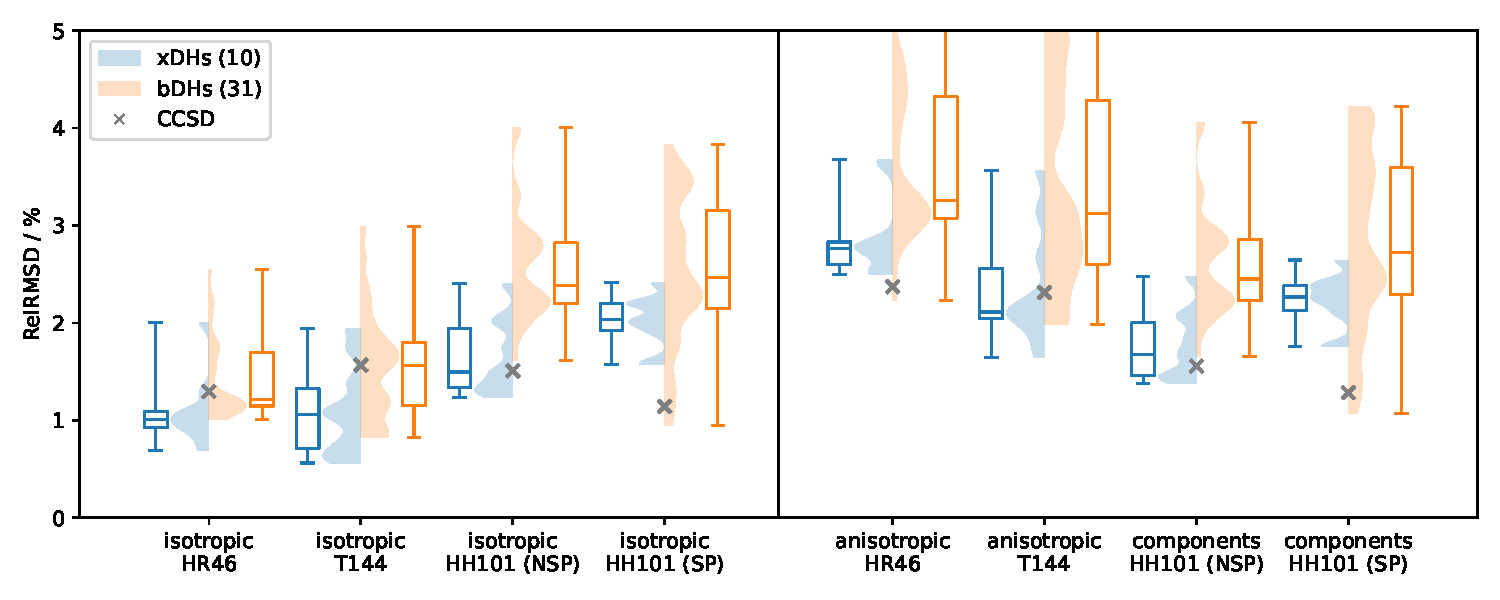
\includegraphics[width=0.8\textwidth]{assets/benchmark-compare-xdh-bdh.pdf}
    \caption[xDH 与 bDH 极化率 RelRMSD 测评表现与对比图]{诸 XYG3 型双杂化泛函 (xDH) 与诸 B2PLYP 型双杂化泛函 (bDH) 泛函极化率数据集相对方均根误差 (RelRMSD) 测评表现图。图例参考图 \ref{fig.6.benchmark-compare-dh-low}。}
    \label{fig.6.benchmark-compare-xdh-bdh}
\end{figure}

随后对不同类型的双杂化的误差作更细致的讨论。图 \ref{fig.6.benchmark-compare-xdh-bdh} 展示了 xDH 型泛函与 bDH 型泛函误差的比较示意图。可以看到,对于 HR46 同性极化率 $\alpha$、T144 数据集以及 HH101 自旋非极化分子子集,比之于 bDH 型泛函,xDH 型泛函的总体表现与最低误差都更好。作为特例,在 HR46 异性极化率 $\gamma$ 数据集上,DSD-PBEPBE-D3BJ 的 RelRMSD 误差是 2.23\%,比 xDH 型泛函中误差最低的 revXYG3 (2.49\%) 更低一些;但除此泛函以及 DSD-PBEP86-D3BJ (2.56\%) 之外,其余的 bDH 型泛函误差都比除 XYG-OS5 (3.68\%) 外的所有经测评的 xDH 泛函误差更大。因此,我们认为,诸多 xDH 型泛函在 HR46 与 T144 等中等分子的、以自旋非极化体系为主的数据集上,不论是同性极化率 $\alpha$ 还是异性极化率 $\gamma$,都有较为稳定且优异的误差表现。

但 HH101 自旋极化分子子集上,xDH 泛函尽管在平均表现上比 bDH 型泛函更好,但更多的 bDH 型泛函在该数据集上展现出优势。为简化讨论,我们仅考察 HH101 自旋极化子集的同性极化率 $\alpha$ 测评结果。在该数据集上,表现较好的 xDH 型泛函是 XYG7 (1.58\%)、XYGJ-OS (1.59\%)、XYG6 (1.91\%);而 bDH 型泛函中,ωPBEPP86 (0.95\%)、ωB88PP86 (1.13\%)、DSD-PBEP86-D3BJ (1.32\%)、DSD-PBEPBE-D3BJ (1.41\%) 的表现相当出色。除此之外,ωB2GP-PLYP (1.83\%) 也有较好的误差表现。我们注意到,ωPBEPP86、ωB88PP86、ωB2GP-PLYP 等泛函在交换部分包含长短程矫正。

\begin{figure}[!t]
    \centering
    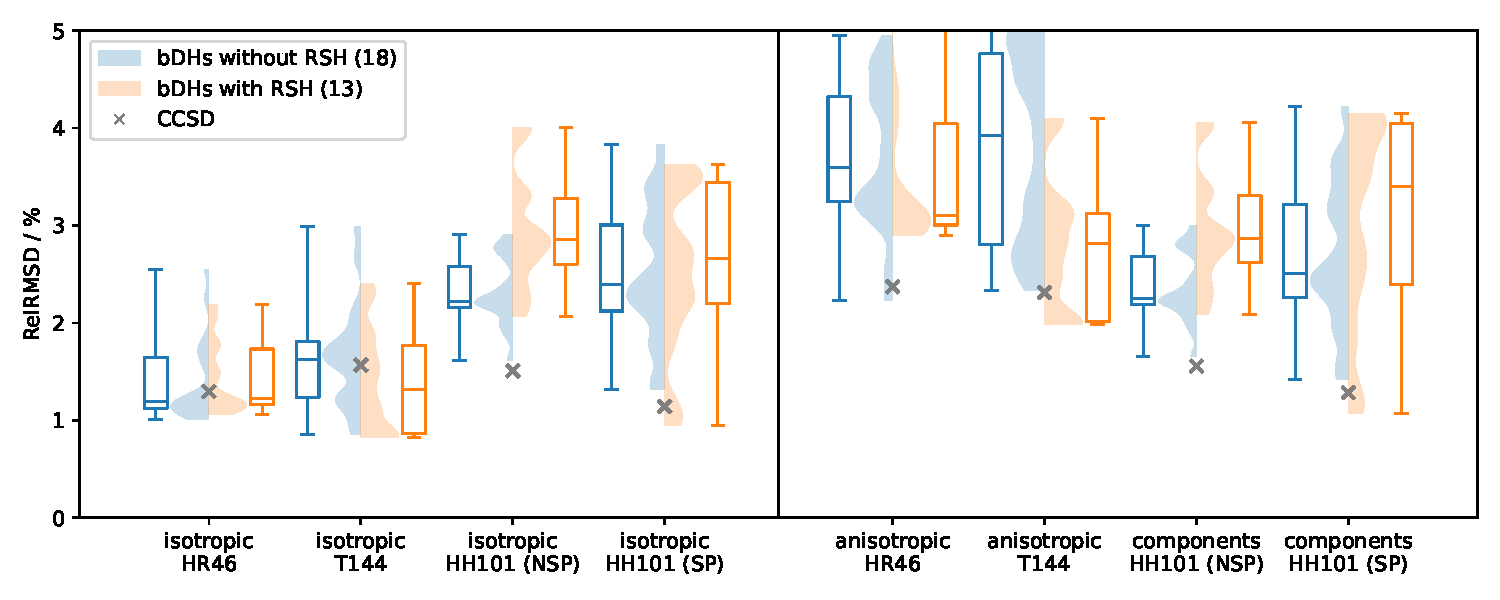
\includegraphics[width=0.8\textwidth]{assets/benchmark-compare-dh-rsh.pdf}
    \caption[bDH 依 RSH 分类的极化率 RelRMSD 测评表现图]{诸 bDH 型双杂化泛函依交换部分是否为 RSH 型泛函而分类的极化率数据集相对方均根误差 (RelRMSD) 测评表现图。图例参考图 \ref{fig.6.benchmark-compare-dh-low}。}
    \label{fig.6.benchmark-compare-dh-rsh}
\end{figure}

由于本工作不涉及交换部分 RSH 型的 xDH 型泛函,因此这里在测评交换部分 RSH 对极化率误差表现时,我们仅考察 bDH 型双杂化泛函。误差表现展示于图 \ref{fig.6.benchmark-compare-dh-rsh}。可以发现,RSH 项的引入确实提升了部分泛函在 HH101 自旋非极化数据集的测评表现,但交换部分 RSH 型泛函总体表现并非总是比非 RSH 型泛函更具有优势。我们还发现,交换部分 RSH 型泛函的测评表现与泛函的构成风格有较大关系:
\begin{itemize}[nosep]
    \item RSX-QIDH、SOS-RSX-PBE-QIDH 等泛函是非参数优化的泛函;它们的表现相对一般;
    \item ωPBEPP86、ωB88PP86、ωB2GP-PLYP、ωB2PLYP 等泛函是专门针对激发态计算所优化;这些泛函在 HH101 数据集上有较好的表现;
    \item RS-B88-LYP、RS-PBE-PBE、RS-PBE-P86、RS-PW91-PW91 等泛函也专门针对激发态作优化,但在泛函形式上还包含相关部分 RSH 的贡献;这些泛函在 T144 数据集上有较好的表现,但在 HH101 自旋极化子集上表现较差。
\end{itemize}
因此,尽管对双杂化泛函引入 RSH 项,确实可以提升部分静态极化率数据集的评测表现;但 RSH 项并非唯一的影响因素、也并非能保证在所有静态极化率计算问题上有所提升。

\section{xDH@B3LYP 模型静态极化率参数优化}
\label{sec.6.pol-xdh-optimize}

\begin{sidewaystable}
\centering
\caption[以静态极化率 WTRE 量标优化的 xDH@B3LYP 参数与测评结果]{以 WTRE 误差量标优化的 xDH@B3LYP 模型静态极化率参数,及各静态极化率数据集误差结果${}^a$。}
\label{tab.6.xdh-b3lyp-polar-opt}
\widetabular{
    \begin{tabular}{lld{2.7}d{2.7}d{2.7}d{2.7}d{2.7}d{2.7}d{2.7}d{2.7}}
    \toprule
    & & \multicolumn{1}{c}{B3LYP} & \multicolumn{1}{c}{XYG3} & \multicolumn{1}{c}{XYG5} & \multicolumn{1}{c}{XYG6} & \multicolumn{1}{c}{XYG7} & \multicolumn{1}{c}{XYG-OS3} & \multicolumn{1}{c}{XYGJ-OS} & \multicolumn{1}{c}{XYG-OS5} \\
    \midrule
    泛函参数\tnote{b}
    & $a_1$ ($E_\textmt{x}^\textmt{exact}$) & 0.330646   & 0.887385   & 0.843480   & 0.707769   & 0.714877  & 0.794151 & 0.667163   & 0.681864   \\
    & $a_2$ ($E_\textmt{x}^\textmt{S}$) & [0.113675] & [0.297922] & [0.231657] & [0.520989] & 0.523649  & [0.205849] & [0.332837] & [0.338714] \\
    & $a_3$ ($E_\textmt{x}^\textmt{B88}$) & 0.555679   & -0.185307  & -0.075137  & -0.228758  & -0.259884 & [0.{\color{white}000000}]     & [0.{\color{white}000000}] & -0.020578  \\
    & $a_4$ ($E_\textmt{c}^\textmt{VWN3}$) & [0.741727] & [0.{\color{white}000000}] & [0.{\color{white}000000}] & 0.995154   & 1.271473  & [0.{\color{white}000000}] & 0.883246   & 1.120226   \\
    & $a_5$ ($E_\textmt{c}^\textmt{LYP}$) & 0.258273   & [0.659253] & 0.615211   & -0.667102  & -0.811699 & 0.673447 & -0.500754  & -0.614148  \\
    & $a_6$ ($E_\textmt{c}^\textmt{OS-PT}$) & [0.{\color{white}000000}] & 0.340747   & 0.408184   & 0.365681   & 0.371477  & 0.419592 & 0.353082   & 0.359351   \\
    & $a_7$ ($E_\textmt{c}^\textmt{SS-PT}$) & [0.{\color{white}000000}] & [0.340747] & 0.115199   & 0.049551   & 0.038238  & [0.{\color{white}000000}] & [0.{\color{white}000000}] & [0.{\color{white}000000}] \\
    \midrule
    同性极化率\tnote{c}
    & HR46        & 1.365      & 0.926      & 0.739      & 0.560      &0.553     & 0.720    & 0.637      & 0.661      \\
    & T144        & 2.102      & 1.004      & 0.729      & 0.794      &0.784     & 0.668    & 0.875      & 0.867      \\
    & HH101 (NSP) & 2.307      & 1.341      & 0.815      & 0.879      &0.971     & 0.913    & 0.800      & 0.853      \\
    & HH101 (SP)  & 3.577      & 2.158      & 2.035      & 1.288      & 1.106     & 2.118    & 1.281      & 1.123      \\ \midrule
    异性极化率\tnote{c}
    & HR46        & 5.201      & 2.185      & 2.238      & 2.290      &2.322     & 2.565    & 2.537      & 2.585      \\
    & T144        & 6.007      & 2.343      & 1.826      & 2.252      & 2.205     & 1.853    & 2.431      & 2.367      \\ \midrule
    极化率分量\tnote{c}
    & HH101 (NSP) & 2.398      & 1.431      & 0.998      & 1.020      &1.131     & 1.118    & 0.942      & 1.003      \\
    & HH101 (SP)  & 3.725      & 2.395      & 2.237      & 1.418      & 1.240     & 2.306    & 1.410      & 1.259      \\ \midrule
    WTRE\tnote{d}
                &             & 0.884      & 0.471      & 0.388      & 0.347      & 0.342     & 0.405    & 0.360      & 0.356      \\ \bottomrule
    \end{tabular}
}{
    \item[a] 该表格的泛函名称 (如 B3LYP、XYG7 等) 并不指代业已发表的泛函,而是指代其对应的参数模型。B3LYP 参数模型参考 Stephens 等人工作\cite{Stephens-Frisch.JPC.1994},XYG-OS3 为本工作的参数模型,其余参数模型参考张颖与徐昕的工作\cite{Zhang-Xu.JPCL.2021}。
    \item[b] 该参数表的定义参考张颖与徐昕的工作\cite{Zhang-Xu.JPCL.2021},或参考表 \alertref{tab.2.coeff-xyg6-1-weighted-error}。
    \item[c] 测评误差以 RelRMSD (\%) 表示。
    \item[d] 加权相对误差的定义参考式 (\ref{eq.6.wtre}) 附近的讨论。
}
\end{sidewaystable}

这一节将基于 xDH@B3LYP 参数化模型\cite{Zhang-Xu.JPCL.2021},仅针对极化率测评表现进行参数优化。需要指出,本节所涉及的泛函名称 (如 XYG7、B3LYP 等) 可能指代其对应的参数化模型,而并非指代业已发表的泛函本身。本节的参数优化仅适用于静态极化率测评与分析;既不额外引入基于能量或结构等测评结果、也未引入对泛函公式形式的物理限制的前提下,我们认为这里的泛函参数优化过程并非是对普适泛函的一种逼近策略。

表 \ref{tab.6.xdh-b3lyp-polar-opt} 展示了针对极化率的加权相对误差量标 WTRE,xDH@B3LYP 模型下的参数优化结果与测评误差。可以看到,
\begin{itemize}[nosep]
    \item 原始的 B3LYP 泛函的 WTRE 误差为 1.647;而对 B3LYP 三参数模型作优化后,其 WTRE 误差降低到 0.884,与本工作所被测评的最好的低阶泛函 MPW1K 的 WTRE 误差 0.877 较为接近。这一方面表明,对于类似于 B3LYP 的低阶泛函,其极化率表现可以通过参数重新优化得到大幅提升;但另一方面,在没有引入二阶微扰贡献的前提下,即使放开 B3LYP 的三参数优化,也难以达到普通双杂化泛函的极化率计算误差表现。这加强了先前泛函测评得到的结论,即双杂化泛函的表现明显优于低阶泛函。
    \item 除 XYG3 之外,其余 xDH@B3LYP 泛函的参数化模型都可以优化得到 0.41 以下的 WTRE (在表 \ref{tab.6.full-benchmark} 所测评的泛函中,表现最好的是 XYGJ-OS,其 WTRE 为 0.418)。这意味着放开部分或所有 xDH@B3LYP 模型参数确实可以提升静态极化率测评表现。但同时需要指出,当放开所有参数时,XYG7 参数化模型的 WTRE 误差仍然有 0.342;该误差并未比原始的 XYGJ-OS 泛函误差 0.418 小许多。因此,对 xDH@B3LYP 模型参数放开优化确实有所提升,但提升较为有限。
    \item 对于同时放开 VWN3 型相关能参数 $a_4$ 与 LYP 型相关能参数 $a_5$ 的情形 (XYG6, XYG7, XYGJ-OS, XYG-OS5 四种模型),参数 $a_5$ 的数值会产生相当严重的负值、同时参数 $a_4$ 有较大的数值;这些参数化模型给出的 WTRE 误差也相对较小 (在 0.34--0.36 之间)。但考虑到 xDH@B3LYP 参数化模型在对诸如 GMTKN55 等反应能误差量标下,参数优化很少遇到这种严重负值的情形;且同时放开 $a_4$ 与 $a_5$ 参数优化的极化率测评 WTRE 误差表现并不显著地比冻结其中一者优化的情形有优势 (XYG5 模型或 XYG-OS3 模型的误差在 0.38--0.41 之间);因此我们担忧,过度放开参数优化限制、且仅针对极化率问题作参数优化,尽管在 WTRE 量标上有微少的提升,但却会导出偏离物理图像或直觉的泛函。
    \item 在放开同自旋二阶微扰贡献项 $E_\textmt{c}^\textmt{SS-PT}$ 的 $a_7$ 参数模型中 (XYG5, XYG6, XYG7 三种模型),所有优化得到的 $a_7$ 参数接近零值 (均小于 0.12)。而若将 $a_7$ 参数置零,如 XYG-OS5 模型之于 XYG6 模型,误差不会显著地提升。而对比 XYG3 模型与 XYG-OS3 模型,可以发现同样为三参数模型,XYG-OS3 模型静默 $a_7$ 参数的 WTRE 误差 0.41 明显小于 XYG3 模型的 0.47。因此,限制 $E_\textmt{c}^\textmt{SS-PT}$ 的贡献、或合理地分离二阶微扰的两种自旋贡献 $E_\textmt{c}^\textmt{OS-PT}$ 与 $E_\textmt{c}^\textmt{SS-PT}$,可以有效地提升极化率测评表现。
\end{itemize}

\section{讨论与本章小结}

基于对双杂化泛函极化率测评的目的,本章展开了一系列分析、验证与测评工作。

为确认一种高效且具有足够精度的计算基组,我们以 B2PLYP 泛函作为双杂化泛函的典型,作细致的基组收敛性分析;并最终估计 aug-pc-3 基组作为计算代价较小的基组,其同性极化率 $\alpha$ 或异性极化率 $\gamma$ 的 BSIE 误差在 0.5\% 误差范围内。我们认为,以该基组作为双杂化或低阶泛函的静态极化率测评是合适的。

我们对诸多双杂化与低阶泛函,对 HR46、T144、HH101 三个数据集的同性极化率 $\alpha$,HR46 与 T144 两个数据集的异性极化率 $\gamma$,以及 HH101 数据集极化率分量 $\alpha_{xx}, \alpha_{yy}, \alpha_{zz}$ 作系统的测评。这部分测评表明,双杂化泛函的极化率误差显著地小于低阶泛函的误差;且表现最优异的双杂化泛函,在以 CCSD(T) 为基准的前提下,其误差可以媲美波函数方法 MP2、或计算开销上更为昂贵 CCSD 或甚至更小。双杂化泛函适合用于以 HR46、T144、HH101 为代表的一系列中小分子的静态极化率计算;而在其中,以 XYGJ-OS、XYG6、xDH-PBE0 为代表的 xDH 型泛函,与 DSD-PBEPBE-D3BJ 为代表的 bDH 型泛函,在各极化率数据集上有相当低的误差表现,是适合用于静态极化率计算的双杂化泛函。

本工作还对各种 xDH@B3LYP 模型下的泛函作参数优化的尝试。我们发现,异自旋二阶微扰贡献项 $E_\textmt{c}^\textmt{OS-PT}$ 对于静态极化率的描述有重要的作用;即在合理的泛函构造下,双杂化泛函确实比专门针对极化率作参数优化的低阶泛函,有更低的误差。同时,当同自旋二阶微扰贡献项 $E_\textmt{c}^\textmt{SS-PT}$ 贡献相比于 $E_\textmt{c}^\textmt{OS-PT}$ 较少甚至于零贡献时,双杂化泛函的极化率误差通常较小。专门针对静态极化率而优化的 xDH@B3LYP 模型泛函确实有更好的极化率表现,但也容易产生非物理或不符合直觉的泛函参数,测评误差的提升也比较有限;考虑到密度泛函的泛用性,我们认为使用以 XYGJ-OS、XYG6、xDH-PBE0、DSD-PBEPBE-D3BJ 为代表的基于能量误差量标优化的泛函,也可以很好地描述静态极化率。